\documentclass{amsart}
\usepackage{amsmath, amsthm, amssymb, amscd}
\usepackage{color}
\usepackage{tikz-cd}
\usetikzlibrary{shapes.geometric}

\begin{document}

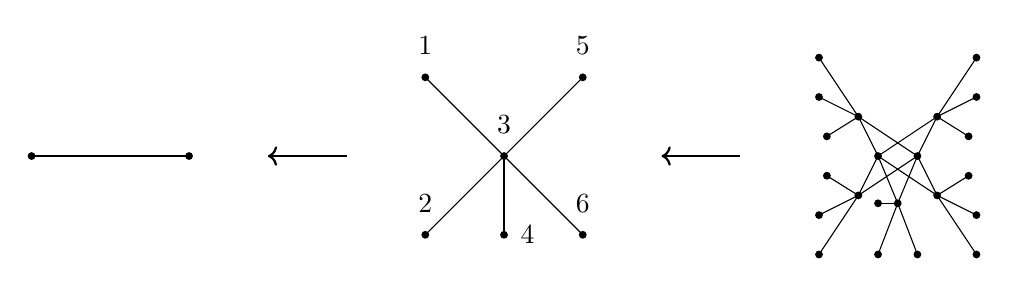
\begin{tikzpicture}[scale=1]
\draw (-6,0)--(-4,0);
\draw[<-,thick] (-3,0)--(-2,0);

\draw (-1,1)--(0,0)--(1,1);
\draw (-1,-1)--(0,0)--(1,-1);
\draw (0,0)--(0,-1);
\draw[<-,thick] (2,0)--(3,0);

\draw (4,1.25)--(4.5,0.5)--(5.25,0);
\draw (4,0.75)--(4.5,0.5)--(4.75,0);
\draw (4.5,0.5)--(4.1,0.25);
\draw (4,-1.25)--(4.5,-0.5)--(4.75,0);
\draw (4,-0.75)--(4.5,-0.5)--(5.25,0);
\draw (4.5,-0.5)--(4.1,-0.25);

\draw (5.25,0)--(5.5,0.5)--(6,1.25);
\draw (4.75,0)--(5.5,0.5)--(6,0.75);
\draw (5.5,0.5)--(5.9,0.25);
\draw (5.25,0)--(5.5,-0.5)--(6,-1.25);
\draw (4.75,0)--(5.5,-0.5)--(6,-0.75);
\draw (5.5,-0.5)--(5.9,-0.25);

\draw (5.25,0)--(5,-0.6)--(4.75,-1.25);
\draw (4.75,0)--(5,-0.6)--(5.25,-1.25);
\draw (5,-0.6)--(4.75,-0.6);

\foreach \p in {(-4,0),(-6,0),(-1,1),(0,0),(1,1),(1,-1),(-1,-1),(0,-1),
(4,1.25),(4.5,0.5),(4,0.75),(4.5,-0.5),(4,-0.75),(4,-1.25),(5.25,0),(4.75,0),(5.5,0.5),(5.5,-0.5), (6,1.25) , (6,0.75),(6,-0.75), (6,-1.25),
(4.75,-0.6),(5,-0.6),(4.75,-1.25),(5.25,-1.25),(5.9,-0.25),(5.9,0.25),(4.1,-0.25),(4.1,0.25)}
\node at \p [circle,fill,inner sep=1pt]{};

\node at (-1,1.4) {1};
\node at (-1,-0.6) {2};
\node at (0,0.4) {3};
\node at (0.3,-1) {4};
\node at (1,1.4) {5};
\node at (1,-0.6) {6};
\end{tikzpicture}

\end{document}